\documentclass[10pt,a4paper]{article}
\usepackage[margin=18mm,top=18mm,bottom=18mm]{geometry}
\usepackage[T1]{fontenc}
\usepackage{helvet}
\renewcommand{\familydefault}{\sfdefault}
\usepackage{amsmath,amssymb,graphicx,booktabs,tabularx,xcolor,microtype,fancyhdr}
\usepackage[colorlinks=true,urlcolor=teal,linkcolor=teal]{hyperref}
\hypersetup{pdftitle={IRMF with pimf versus AS222-style FFT},pdfsubject={Reproduction of the supplied five-sine benchmark with pimf 0.4.0}}
\definecolor{navy}{HTML}{17354E}
\definecolor{teal}{HTML}{007C91}
\definecolor{muted}{HTML}{516578}
\setlength{\parindent}{0pt}
\setlength{\parskip}{5pt}
\setlength{\headheight}{14pt}
\pagestyle{fancy}\fancyhf{}
\renewcommand{\headrulewidth}{0pt}
\renewcommand{\footrulewidth}{0.3pt}
\fancyfoot[L]{\footnotesize\color{muted}pimf / AS222-style FFT \enspace | \enspace Five-sine reproduction}
\fancyfoot[R]{\footnotesize\color{muted}\thepage}
\newcommand{\heading}[1]{\vspace{7pt}{\large\color{teal}#1}\par\vspace{2pt}}
\newcommand{\pagetitle}[1]{{\LARGE\color{navy}#1}\par\vspace{4pt}}
\begin{document}
{\footnotesize\color{muted}RESEARCH COMPARISON \hfill 13 October 2026}\par\vspace{6pt}
\pagetitle{IRMF with \texttt{pimf} versus AS222-style FFT}
{\color{muted}The supplied five-sine benchmark, reproduced with \texttt{pimf 0.4.0}.}

\heading{Result}
The package reproduces all 25 source-report accuracy entries within their displayed rounding.
The FFT comparator still fails the agreement checkpoint in all 100 component pairs.
At $n=1000$, \texttt{pimf} takes \textbf{39.29\,ms with 16 workers}, versus
12.99\,ms with one worker and 0.231\,ms for FFT.
Using all cores slows this small problem; at $n=8000$, it gives a \textbf{5.51-fold speedup}.

\heading{Same experiment, packaged local solver}
Use $t_i=i/n$, $n=1000$, and
\[
Y_i=\sum_{j=1}^{5} w_j\sin(2\pi f_jt_i)+\varepsilon_i,
\qquad \varepsilon_i\overset{\mathrm{iid}}{\sim}N(0,0.2^2).
\]
\begin{minipage}[t]{0.45\linewidth}
\vspace{0pt}
\centering\small
\begin{tabular}{rrrr}
\toprule Component & $f_j$ & $w_j$ & $h_j$\\\midrule
1 & 1 & 0.30 & 0.10000 \\
2 & 3 & 0.25 & 0.08290 \\
3 & 8 & 0.20 & 0.03030 \\
4 & 20 & 0.15 & 0.01280 \\
5 & 50 & 0.10 & 0.00757 \\
\bottomrule
\end{tabular}
\end{minipage}\hfill
\begin{minipage}[t]{0.51\linewidth}
\vspace{0pt}
\small
20 paired realizations; seed 20261004; one validation draw first.
Classical Epanechnikov weights, periodic boundaries, robustness $H=1$.
Each method subtracts its own component before the next bandwidth.
No retuning or contamination is added.
\end{minipage}

\texttt{pimf} uses \texttt{IMF}, \texttt{SmoothAbs(1)}, and \texttt{Epanechnikov()}.
One public \texttt{decompose(..., h1=h, k\_max=1)} call per bandwidth preserves the
nongeometric schedule and its exact fractional widths. Settings are
\texttt{lookup=True}, \texttt{tol=1e-6}, \texttt{max\_iter=60}, and \texttt{workers=16}.

\heading{Component agreement and true-sine recovery}
\small
\begin{center}
\begin{tabular}{rrrrrr}
\toprule
Component / $f$ & $r(P,F)$ & RMS$(P-F)$ & Relative RMS & $r(P,T)$ & $r(F,T)$\\\midrule
1 / 1 & 0.9937 & 0.04001 & 16.8\% & 0.8562 & 0.7947 \\
2 / 3 & 0.8006 & 0.02896 & 64.9\% & 0.9581 & 0.6657 \\
3 / 8 & 0.9921 & 0.03105 & 27.0\% & 0.9727 & 0.9643 \\
4 / 20 & 0.9464 & 0.02741 & 34.0\% & 0.8631 & 0.8890 \\
5 / 50 & 0.9129 & 0.02330 & 49.2\% & 0.6997 & 0.7704 \\
\bottomrule
\end{tabular}
\end{center}
\normalsize
$P$: \texttt{pimf}; $F$: FFT; $T$: corresponding weighted true sine.
Entries average metrics computed separately for each realization.
Relative RMS is $\operatorname{RMS}(P-F)/\operatorname{RMS}(P)$.
The inherited checkpoint requires $r(P,F)\geq0.995$ and relative RMS $\leq5\%$
in \emph{every} pair. It fails, so the conditional 1,000-run extension is not triggered.

\heading{Why changing the implementation does not close the gap}
Let $K$ be the common discrete kernel smoother and
$\psi_H(u)=\operatorname{erf}(u/(\sqrt{2}H))$.
Direct IRMF solves $\sum_iq_{ti}\psi_H(R_i-x_t)=0$.
The comparator instead uses
\[
p=KR,\qquad S=p+\frac{K\psi_H(R-p)}{K\psi'_H(R-p)}.
\]
Its scores are centered at observation-specific pilots $p_i$.
For a linear score, it reduces to $(2K-K^2)R$, whereas direct smoothing gives $KR$.
The discrepancy is in the estimator; FFT arithmetic is accurate.

\newpage
\pagetitle{Recovered components}
{\color{muted}Same observations and bandwidths; each method uses its own residual recursion.}
\begin{center}
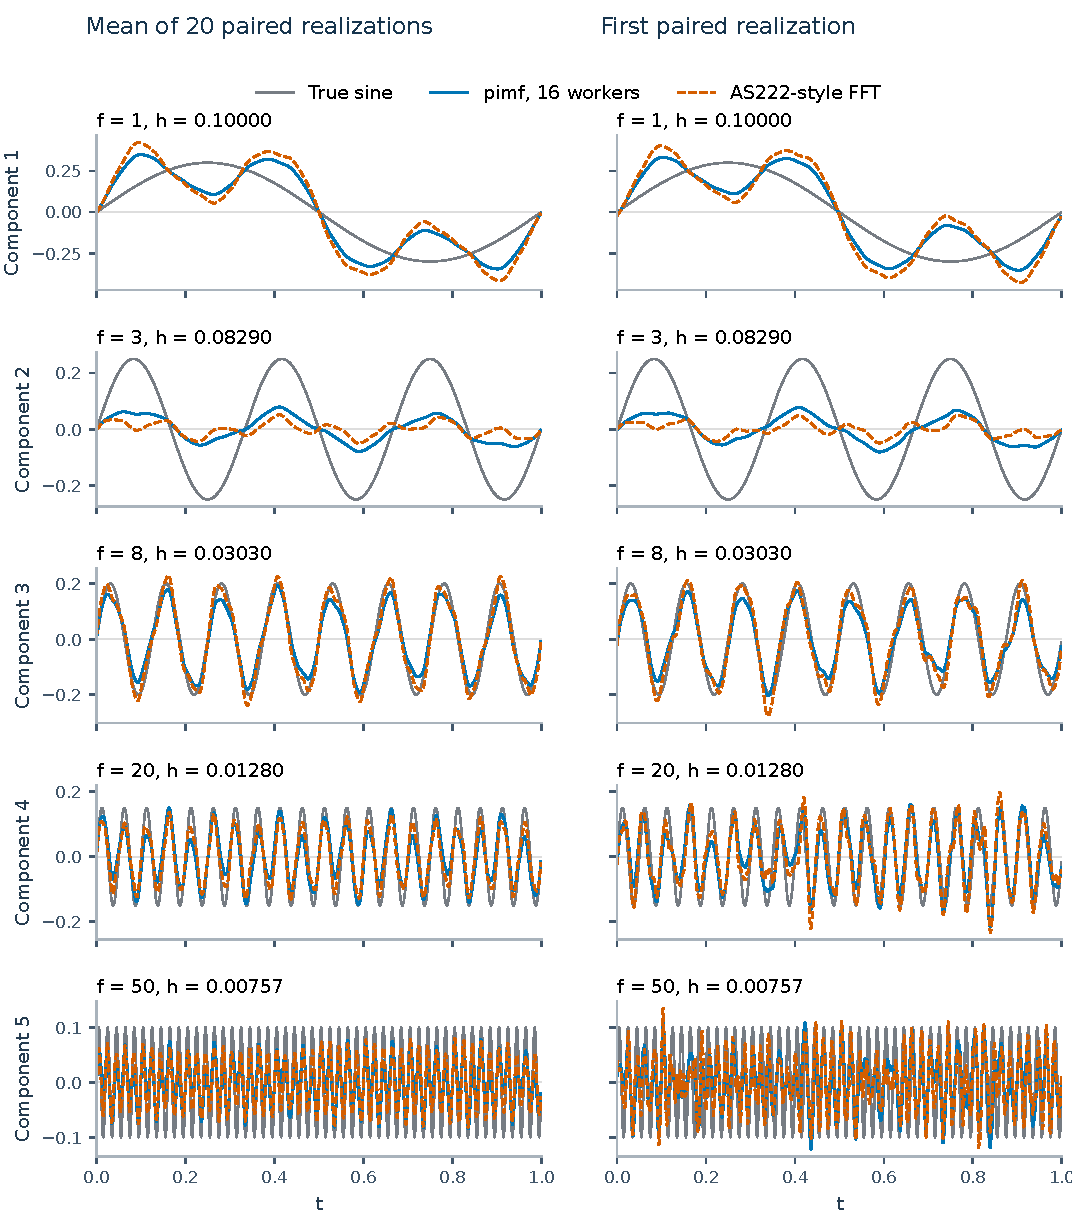
\includegraphics[width=\linewidth]{figures/pimf-as222/components.pdf}
\end{center}
Component 2 has the largest relative disagreement, 64.9\% on average.
The mean curves expose persistent attenuation and leakage; the single-run curves show noise variation.
The correlations on page 1 are per-realization averages, not correlations of the mean curves.

\newpage
\pagetitle{Runtime, checks, and original sources}
\heading{Fresh timing measurements}
\begin{minipage}[c]{0.49\linewidth}
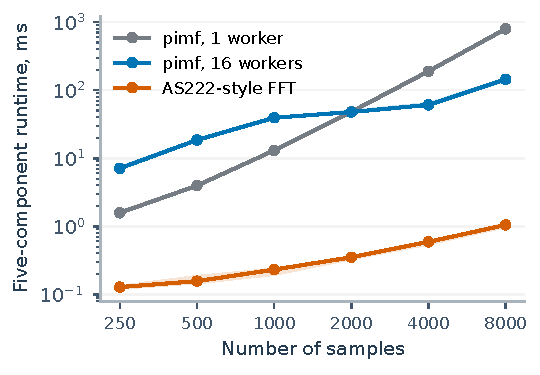
\includegraphics[width=\linewidth]{figures/pimf-as222/runtime.pdf}
\end{minipage}\hfill
\begin{minipage}[c]{0.48\linewidth}
\centering\footnotesize\setlength{\tabcolsep}{4pt}
\begin{tabular}{rrrrr}
\toprule $n$ & 1 worker & 16 workers & FFT & Speedup\\\midrule
250 & 1.58 & 7.10 & 0.128 & 0.22$\times$ \\
500 & 3.95 & 18.50 & 0.156 & 0.21$\times$ \\
1,000 & 12.99 & 39.29 & 0.231 & 0.33$\times$ \\
2,000 & 47.94 & 47.61 & 0.350 & 1.01$\times$ \\
4,000 & 189.15 & 60.75 & 0.590 & 3.11$\times$ \\
8,000 & 793.37 & 143.88 & 1.045 & 5.51$\times$ \\
\bottomrule
\end{tabular}
\par\vspace{4pt}Times in ms; speedup = 1-worker / 16-worker time.
\end{minipage}

Five warmed repetitions per size, with all three configurations retimed in randomized order.
Timing includes five smoothing calls, thread-pool creation, and residual updates. Kernel weights
and FFT spectra are precomputed; simulation, setup, checks, and plotting are excluded.
Shading shows the observed range. Cached and uncached package outputs are bit-identical.

Apple M4 Max, 16 cores; Python 3.14.6; NumPy 2.5.4; SciPy 1.18.1.
Numerical-library threads remain at one. \texttt{workers=16} gives pool capacities of 4, 8,
and 16 for $n=250$, $500$, and $n\geq1000$, because \texttt{pimf} requires at least 64 samples
per chunk. Parallel overhead outweighs gains at small $n$; all measured FFT times remain lower.

\heading{Numerical checks}
\small
\begin{tabularx}{\linewidth}{@{}Xr@{}}
\toprule Check & Maximum absolute error\\\midrule
16-worker \texttt{pimf} versus 25 exact-score Brent roots & $1.28\times 10^{-7}$\\
FFT versus spatial evaluation of the same one-step formula & $2.22\times 10^{-16}$\\
Package versus independently sampled kernel weights & $2.08\times 10^{-17}$\\
Default package versus tighter solver with score lookup disabled & $1.69\times 10^{-7}$\\
Reconstruction across all 20 paired runs & $4.44\times 10^{-16}$\\
One versus 16 workers across all 20 paired runs & $1.34\times 10^{-7}$\\
\bottomrule
\end{tabularx}
\par\vspace{3pt}
\normalsize
All 100 parallel package stages converged, with at most 7 iterations.
Thread chunks stop independently, explaining small differences near solver tolerance.
The root and tight-solver checks use the separate validation realization.

\heading{What the original papers establish}
H\"ardle's AS222 paper is from \textbf{1987}; the \textbf{1988} paper is Dusoir's correction.
Equation 2 of AS222 gives the pilot-plus-score-ratio construction, using Huber scores and Gaussian
smoothing. Page 106 explicitly notes the changed score centers. Dusoir corrects initialization
of \texttt{WK(5:6,:)} and \texttt{M1=M/2}. Both full publisher PDFs were retrieved and checked.

This experiment preserves the supplied report's Gaussian-score, Epanechnikov-kernel adaptation,
with an unbinned periodic grid. It does not reproduce historical Fortran outputs or the original
contaminated random-design example. Modern kernel transforms are explicitly initialized and inverse
FFTs specify their length. Twenty Gaussian-noise realizations establish this comparison only;
they do not test resistance to outliers or automatic bandwidth selection.

\heading{Reproduce and inspect}
\small
The experiment README at \path{experiments/pimf-as222/README.md} gives the commands and
pinned dependencies. Raw paired metrics, timing repetitions, curves, solver diagnostics,
checks, and source hashes are in \path{output/pimf-as222/}.

\vspace{3pt}
\textbf{Sources.} Supplied comparison PDFs dated 4 and 8 October 2026.
W. H\"ardle, \emph{Resistant Smoothing Using the Fast Fourier Transform}, 1987, 36:104--111,
\href{https://doi.org/10.2307/2347850}{doi:10.2307/2347850}.
T. Dusoir, \emph{Remark AS R73}, 1988, 37:316--317,
\href{https://doi.org/10.2307/2347358}{doi:10.2307/2347358}.
\href{https://pypi.org/project/pimf/0.4.0/}{pimf 0.4.0, PyPI}.
The source reports' code and saved arrays were not supplied; matching their rounded tables
does not establish bitwise reproduction of their curves.
\end{document}
